%%%%%%%%%%%%%%%%%%%%%%%%%%%%%%%%%%%%%%%%%
% Short Sectioned Assignment
% LaTeX Template
% Version 1.0 (5/5/12)
%
% This template has been downloaded from:
% http://www.LaTeXTemplates.com
%
% Original author:
% Frits Wenneker (http://www.howtotex.com)
%
% License:
% CC BY-NC-SA 3.0 (http://creativecommons.org/licenses/by-nc-sa/3.0/)
%
%%%%%%%%%%%%%%%%%%%%%%%%%%%%%%%%%%%%%%%%%

%----------------------------------------------------------------------------------------
% PACKAGES AND OTHER DOCUMENT CONFIGURATIONS
%----------------------------------------------------------------------------------------

\documentclass[paper=a4, fontsize=11pt]{scrartcl} % A4 paper and 11pt font size

\usepackage[T1]{fontenc} % Use 8-bit encoding that has 256 glyphs
\usepackage{fourier} % Use the Adobe Utopia font for the document - comment this line to return to the LaTeX default
\usepackage[english]{babel} % English language/hyphenation
\usepackage{amsmath,amsfonts,amsthm} % Math packages
\usepackage[margin=0.7in]{geometry}

\usepackage{sectsty} % Allows customizing section commands
%\allsectionsfont{\centering \normalfont\scshape} % Make all sections centered, the default font and small caps

\usepackage{pgfplots}
\usepackage{tikz} % Работа с графикой
\usepackage{pgfplotstable}
\pgfplotsset{compat=1.3}

\usepackage{hyperref} %hyperlinks
\usepackage{float}
\usepackage{csquotes}
\usepackage{rotating}

\usepackage{color}
\usepackage{amsmath}
\usepackage{booktabs}
\usepackage[framemethod=TikZ]{mdframed}


\usepackage{array}
\newcolumntype{L}[1]{>{\raggedright\let\newline\\\arraybackslash\hspace*{0pt}}m{#1}}
\newcolumntype{C}[1]{>{\centering\let\newline\\\arraybackslash\hspace*{0pt}}m{#1}}
\newcolumntype{R}[1]{>{\raggedleft\let\newline\\\arraybackslash\hspace*{0pt}}m{#1}}

\usepackage{fancyhdr} % Custom headers and footers
\pagestyle{fancyplain} % Makes all pages in the document conform to the custom headers and footers
\fancyhead{} % No page header - if you want one, create it in the same way as the footers below
\fancyfoot[L]{Belino Xhafa, Christopher Chen, Josh Felizardo, \& Wenzhe (Harry) Xue} % Empty left footer
\fancyfoot[C]{} % Empty center footer
\fancyfoot[R]{\thepage} % Page numbering for right footer
\renewcommand{\headrulewidth}{0pt} % Remove header underlines
\renewcommand{\footrulewidth}{0pt} % Remove footer underlines
\setlength{\headheight}{10.6pt} % Customize the height of the header

\numberwithin{equation}{section} % Number equations within sections (i.e. 1.1, 1.2, 2.1, 2.2 instead of 1, 2, 3, 4)
\numberwithin{figure}{section} % Number figures within sections (i.e. 1.1, 1.2, 2.1, 2.2 instead of 1, 2, 3, 4)
\numberwithin{table}{section} % Number tables within sections (i.e. 1.1, 1.2, 2.1, 2.2 instead of 1, 2, 3, 4)

\setlength\parindent{0pt} % Removes all indentation from paragraphs - comment this line for an assignment with lots of text

\usepackage{graphicx}


%----------------------------------------------------------------------------------------
% TITLE SECTION
%----------------------------------------------------------------------------------------

\newcommand{\horrule}[1]{\rule{\linewidth}{#1}} % Create horizontal rule command with 1 argument of height
\newcommand{\prp}{\mathbb{P}}

\title{ 
\normalfont \normalsize 
\textsc{Harvard University, Stat 139, Spring 2016} \\ [25pt] % Your university, school and/or department name(s)
\horrule{0.5pt} \\[0.4cm] % Thin top horizontal rule
\huge Mamba Out: Analyzing Kobe Bryant's Shooting Performance \\ % The assignment title
\horrule{2pt} \\[0.5cm] % Thick bottom horizontal rule
}


\newenvironment{problem}[1]{\par\bigskip\noindent\textbf{Problem git 
#1.}\enskip\ignorespaces}{}

\mdfdefinestyle{MyFrame}{%
    linecolor=black,
    outerlinewidth=0.5pt,
    roundcorner=5pt,
    innertopmargin=\baselineskip,
    innerbottommargin=\baselineskip,
    innerrightmargin=15pt,
    innerleftmargin=15pt,
    backgroundcolor=gray!2!white}

\author{Belino Xhafa, Christopher Chen, Josh Felizardo, \& Wenzhe (Harry) Xue}
\date{\normalsize May 4, 2016} % Today's date or a custom date

\begin{document}

\maketitle % Print the title

\tableofcontents
\section{Research Questions}
\begin{itemize}
	\item What factors influenced whether Kobe Bryant made a given shot? Is Kobe especially talented at a particular type of shot?
	\item Kobe Bryant is a renowned ``clutch'' player. Is there a statistically significant difference between Kobe Bryant's accuracy in clutch versus non-clutch situations?
	\item Is there a statistically significant relationship between Kobe's game performance and the ultimate result of a given game (on average)?
	\item Did his major injuries have a significant impact on his performance in the short/long term?
	\item Did Kobe's performance change depending on whether he was playing at home or away? How about during the playoffs?
\end{itemize}
\section{Motivation}
\hspace*{1cm}Often considered one of the best players in NBA history, Kobe Bryant has become synonymous with many positive aspects of the game of basketball. While known as a prolific volume scorer, Kobe has also built a reputation as an aggressive and clutch player, dictating his team's performance in the closing parts of each game. At the same time, there are many potential factors that could affect his performance in games, such as where he was playing, whether the Lakers won or lost, or whether he was suffering from injuries. In particular, Kobe has also been renowned as a remarkably tough player, so the effects of injuries on his performance would be especially interesting to consider. And given his recent retirement, we believe that researching the factors influencing (and influenced by) Kobe's shooting accuracy will prove to be a useful, relevant, and intriguing application of the statistical techniques learned in this class. 
\section{Hypotheses}
\hspace*{1cm}In terms of Kobe's accuracy for a specific shot, although he is well known for his mid-range and long-range jump shots, we believed that, like many NBA players, Kobe would be significantly better at closer shots i.e. dunks, layups, and tip ins because of their proximity to the basket and his aggressiveness. Moreover, because of his clutch reputation we believed that Kobe would perform significantly better during clutch situations, which we defined as the last two minutes of the fourth quarter as well as any overtime periods. Because of that clutch factor as well as his high-impact, volume scoring playstyle, we further hypothesized that there would be a significant positive relationship between Kobe's performance - in the clutch and overall - and the Lakers' chances of winning a given game. Lastly, because he is also known as a fierce and tough competitor, both mentally and physically, we believed that Kobe's performance would not be significantly affected by injuries, playing in home versus away games, or during playoff games.
\section{Methods}
	\subsection{Dataset Used}
	\hspace*{1cm}The dataset used as the basis for our analysis was downloaded from the Kobe Bryant Shot Selection Kaggle competition \cite{kagglecompetition}.
	\subsection{Overview}
	Our code is divided into the following files as follows:
		\begin{itemize}
			\item \textbf{analysis.R} contains preliminary exploratory analysis of the datasets
			\item \textbf{cleaning.R} contains the commands we ran to clean/preprocess the data
			\item \textbf{hypothesis\_testing.R} contains various hypothesis tests for statistical significance
			\item \textbf{models.R} contains the models we created based on the data
		\end{itemize}
	Datasets:
		\begin{itemize}
			\item \textbf{raw.csv}: Raw data downloaded from Kaggle
			\item \textbf{cleaned.csv}: Processed data with our modifications and dummy variables added
			\item \textbf{clutch\_shots.csv}: Data on Kobe's shooting performance in clutch situations
			\item \textbf{win\_loss.csv}: Win-loss data scraped from \texttt{landofbasketball.com}
		\end{itemize}
	\subsection{Data Preprocessing}
	\hspace*{1cm}Fortunately, since we were dealing with a Kaggle dataset, the data was, for the most part, well-formatted to begin with. The main changes we made in preprocessing were to remove the rows where there was no record of whether a shot was made (these were the rows to be predicted in the Kaggle competition, but were not very useful for our purposes), add dummy variables and add in win-loss data.

	\hspace*{1cm}While preprocessing the data, we thought it would be helpful to normalize the variables for game date and the season to be integers beginning with 1 and increasing by 1 for each successive season/game because we thought it likely that Kobe's skill level changed with time and normalizing the time-dependent variables (using a \texttt{for} loop to increment a counter variable every time we found a unique instance of a time-dependent variable in the date-ordered data set) would allow us to more easily use them as predictors.

	\hspace*{1cm}Additionally, we created a separate data frame specifically to track Kobe's ``clutch'' shots, that is, the shots Kobe attempted when there were less than 2 minutes remaining in the game or during any overtime periods, in order to examine whether Kobe's shooting accuracy improved or suffered towards the end of the game and whether Kobe lived up to his ``clutch'' reputation. We thought 2 minutes was a reasonable threshold for ``clutch'' shooting because the 2 minute mark is close enough to the end of the game to warrant riskier plays but far away enough for Kobe to execute those plays and actually take some shots. Moreover, the stakes in each overtime period can also be considered a clutch time because of the added mental pressure created by the additional period, so taking into account the entirety of each overtime period as part of the clutch category makes sense. We also created a variable to track Kobe's shooting percentage for non-clutch shots to avoid multicollinearity during model building if we were to use Kobe's ``clutch'' shooting percentage as a regresssor.
	\subsection{Addition of Win-loss Data}
	\hspace*{1cm}Unfortunately the Kaggle dataset did not include data on whether the game during which a particular shot took place was won by the Lakers or not. Therefore we decided to gather that data ourselves. We scraped win-loss data for all Lakers games in the time period covered by the Kaggle dataset from \texttt{landofbasketball.com} \cite{landofbasketball} using the ``Web Scraper'' Chrome extension and merged that data with the original Kaggle dataset for use in our analysis.
	\subsection{New Variables Created}
	The following is a list of new columns that we added to the original dataset from Kaggle:
	\begin{itemize}
	\item \texttt{win}: Dummy variable for whether the Lakers won the game.
	\item \texttt{home}: Dummy variable for whether the game was at home or away.
	\item \texttt{three\_pointer}: Dummy variable for whether the shot was a three-pointer.
	\item \texttt{jump\_shot}: Dummy variable for whether the shot was a jump-shot. $0$ indicates a default of layup.
	\item \texttt{dunk}: Dummy variable for whether the shot was a dunk. $0$ indicates a default of layup.
	\item \texttt{tip\_shot}: Dummy variable for whether the shot was a tip-shot. $0$ indicates a default of layup.
	\item \texttt{hook\_shot}: Dummy variable for whether the shot was a hook-shot. $0$ indicates a default of layup.
	\item \texttt{bank\_shot}: Dummy variable for whether the shot was a bank-shot. $0$ indicates a default of layup.

	\item \texttt{game\_date\_formatted}: Reformatted date into R's native format for boolean comparisons during data processing. 
	\item \texttt{game\_number}: Normalized game date. First game is 1, for game $i$, $game\_number[i] = i$.
	\item \texttt{avg}: Average shot percentage for each game.
	\item \texttt{shots\_made}: Shots made for each game (may seem redundant, but useful for calculating averages over multiple games since we can't just average the averages)
	\item \texttt{shots\_taken}: Shots taken per game (may seem redundant, but useful for calculating averages over multiple games since we can't just average the averages)
	\item \texttt{clutch\_threshold}: Number of minutes remaining at which we begin counting shots as clutch shots.
	\item \texttt{clutch\_perc}: Average shooting percentage for clutch shots (shots attempted with less than 2 minutes remaining during the 4th period or during overtime) for each game.
	\item \texttt{clutch\_shots\_made}: number of clutch shots made for each game.
	\item \texttt{clutch\_shots\_taken}: number of clutch shots taken for each game. 
	\item \texttt{non\_clutch\_perc}: Average shooting percentange for non-clutch shots (shots attempted with above \texttt{clutch\_threshold} minutes remaining) for each game. 
	\item \texttt{ot}: dummy variable for whether or not the game went overtime.
	\item \texttt{ot\_taken}: number of shots taken in OT.
	\item \texttt{ot\_made}: number of shots made in OT.
	\item \texttt{ot\_avg}: OT shooting percentage for each game.
	\item \texttt{season\_norm}: represents the number of seasons Kobe has been in the NBA at the time of each game.

	\end{itemize}
\section{Assumptions}
\subsection{Randomness of Data}
\hspace*{1cm}Since our original data is from a Kaggle competition, not all of Kobe's shots are included ($5000$ are hidden). However we assume that despite the incompleteness of this dataset, the data should still be an accurate representation of overall trends in Kobe Bryant's shooting performance. We believe that this is a reasonable assumption to make since it appears that Kaggle randomly assigns data into its training and testing datasets \cite{forumpost}, so the data we had to work with should be a (very large) random sample of Kobe Bryant's shots.
\section{Results}
\subsection{Exploratory Analysis}
Before creating any models or performing significance tests, we decided to perform some preliminary visualization to better understand Kobe's shooting percentage over period, over season and by shot type. The graphs from initial exploration are as follows, along with our initial reactions prior to performing more in-depth analysis:
\begin{center}
	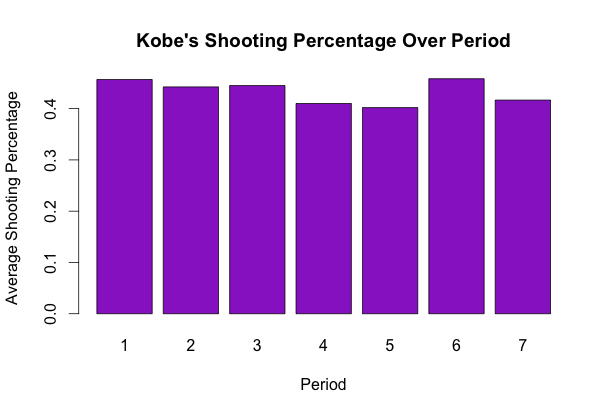
\includegraphics[width=14cm]{img/period}
\end{center}
Note that periods $5$ through $7$ refer to overtime periods. Kobe appears to be relatively consistent in his shooting percentage over the periods. Contrary to our hypotheses, there does not appear to be a marked improvement in his shooting in the latter periods. In fact, his lowest percentages are in the fourth, fifth and seventh periods, though his highest percentage is in the sixth period.  

\begin{center}
	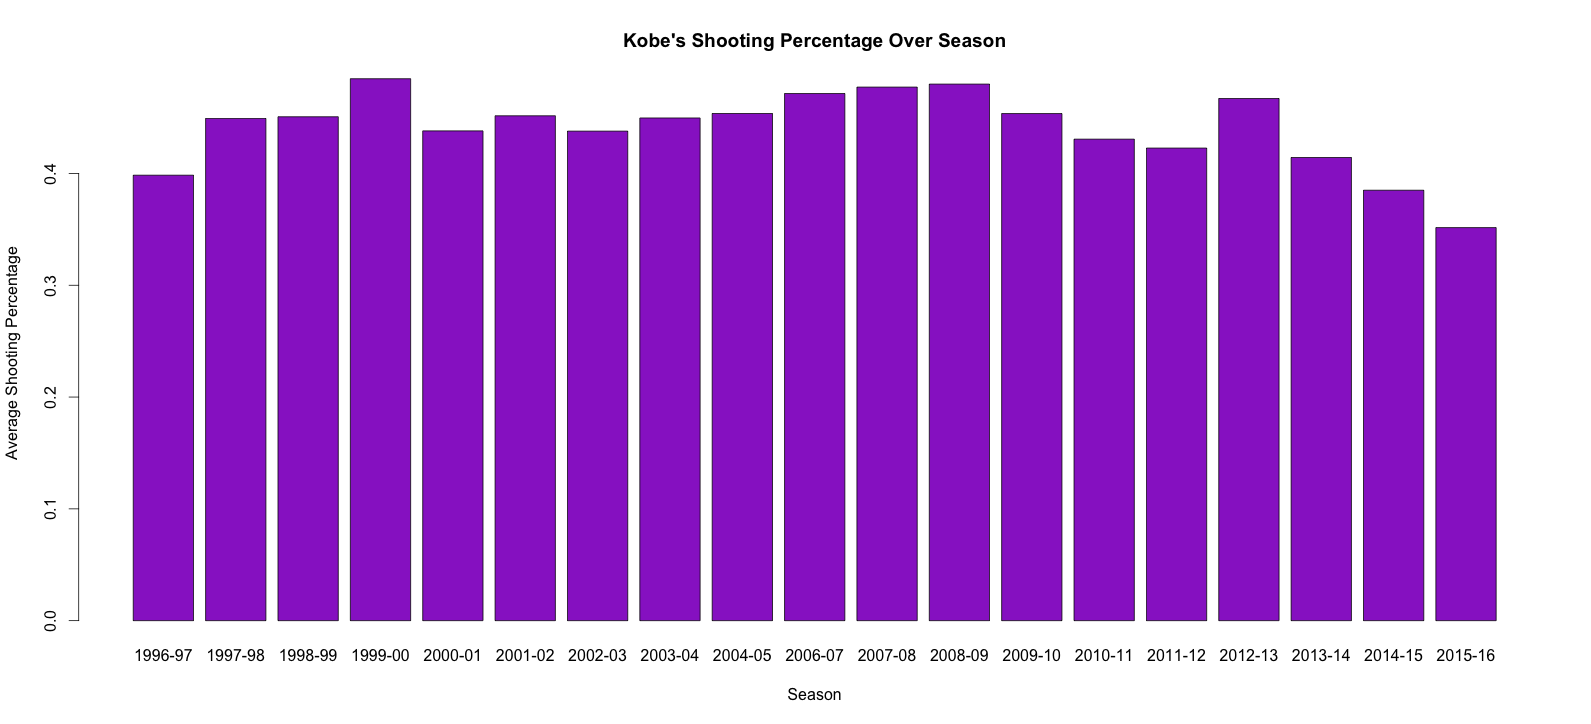
\includegraphics[width=19cm]{img/season}
\end{center}
Consistency again is the main trend when it comes to Kobe's shooting performance over season for most of his career. As expected, there is a noticeable decline in his final few seasons.
\begin{center}
	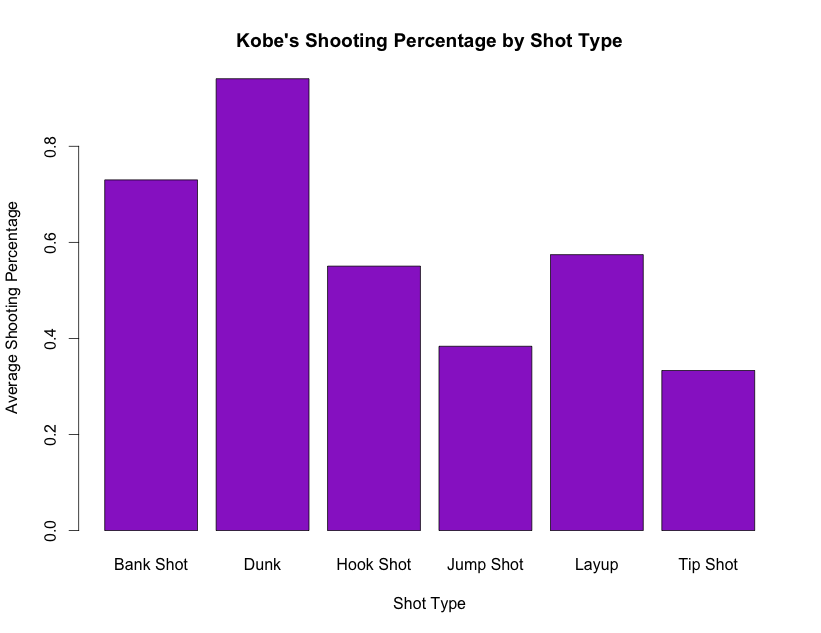
\includegraphics[width=14cm]{img/type}
\end{center}
Unsurprisingly, Kobe's most accurate shot is a dunk given the close range. His second most accurate shot is a bank shot and his least accurate shot is the jump shot, which makes sense given that this category would include three pointers.\\

After making these preliminary observations, we moved on to significance testing and model building.

\subsection{Significance Testing}
\hspace*{1cm}With the dummy variables we inserted into our final datasets there seemed to be a good initial framework for two-sample t-testing to compare Kobe's average field goal percentage i.e. shots made/shots taken in various situations. However, the major assumption of Normality was violated by most of these subsamples of our datasets, so conventional t-testing was not an appropriate approach. To address the Normality concerns we instead chose to take a bootstrapping approach and construct and compare confidence intervals for Kobe's true field goal percentage under different conditions. In essence we created a function that takes in a numerical vector, with 1's representing shots made and 0's representing shots missed, and calculates a confidence interval for the true field goal percentage based on that vector after sampling with replacement 1000 times to create the bootstrapped data \cite{bootstraptheory}. Once we created two 95\% confidence intervals based on our data on Kobe's performance under the different situations, we could check for overlap to see whether there was a significant difference in his performance. For example, we observed that in terms of clutch field goal percentage, Kobe shot significantly better in wins compared to losses, which aligned with our initial hypothesis. Moreover, when comparing his field goal percentage in clutch versus non-clutch situations, we found that Kobe's performance was better in the non-clutch periods, which was hinted at by our exploratory analysis and contrasted with our initial hypothesis. And while we look at Kobe's performance over the long term later to consider the effects of injuries, one of Kobe's most striking examples of enduring injury was in the 2007-2008 season, when he played through a severe injury to his pinky finger on his shooting hand. When comparing his performance before and after the injury occurred in that season, we found no significant change in his overall effectiveness. One thing to note was that although Kobe played through all 82 games of this season, the dataset only contained 55 total games from that time, potentially limiting the significance of our findings. 
\subsection{Model Building and Interpretations}
\subsubsection{Logistic Regression on Shot Made Data}
\hspace*{1cm}After performing some research, we decided to use a logit regression instead of the usual linear regression techniques learned in this class. We made this decision because our response variable (whether or not Kobe made a shot) is a binary variable with only two possibilities: making the shot or missing the shot. The issues involved with using a binary response variable in a normal linear regression include: (1) nonconforming predicted probabilities, (2) constant effects of our regressor variables, and (3) heteroskedasticity. (1) Nonconforming predicted probabilities simply refers to the fact that a linear model could have given us probabilities that are below 0 or above 1 since the predicted values of the response variable generated by a linear model are unconstrained. This would clearly have been an issue because probability values above 1 and below 0 are categorical errors which are impossible to interpret. (2) Constant effects of regressor variables results from the fact that in a linear model, the constant coefficients of each regressor imply that a given regressor will always have the same effect on the predicted outcome regardless of the values of the other regressors, which would have been undesirable for our model. Take the example of Kobe shooting from across the court. Whether or not he was playing against a good team when he took that shot probably would have had an extremely small effect on whether or not he made the shot. However, if he were shooting from a closer distance, the strength of the opposing team could very well have impacted his accuracy. The exponential form of the logit equation allowed for non-constant effects of regressor variables while a linear model would not have. (3) Heteroskedasticity would have resulted from using a linear model because the variance of the error terms would have been directly tied to the probability of observing particular values for any given regressor. Because of the three reasons above, we decided to not use the normal linear regression and opt for a logit regression. 

\hspace*{1cm}We had much fewer and more easily met assumptions about the data with the logit model. These assumptions were: (1) a large sample size, (2) binary dependent variable, (3) no autocorrelation in the dependent variable, (4) independent regressors, and (5) a correctly-fitted model. Our data consisted of 18241 points so we certainly had a large enough sample size to satisfy assumption (1). We observed that the response variable was binary both in theory and as reflected in our data, which satisfied assumption (2). Next, we attempted to check to see if there was any autocorrelation in the dependent variable. We simply looked at the graph (given below) of whether the shot was made or not over time. There did not appear to be any relationship, satisfying assumption (3).
\begin{center}
	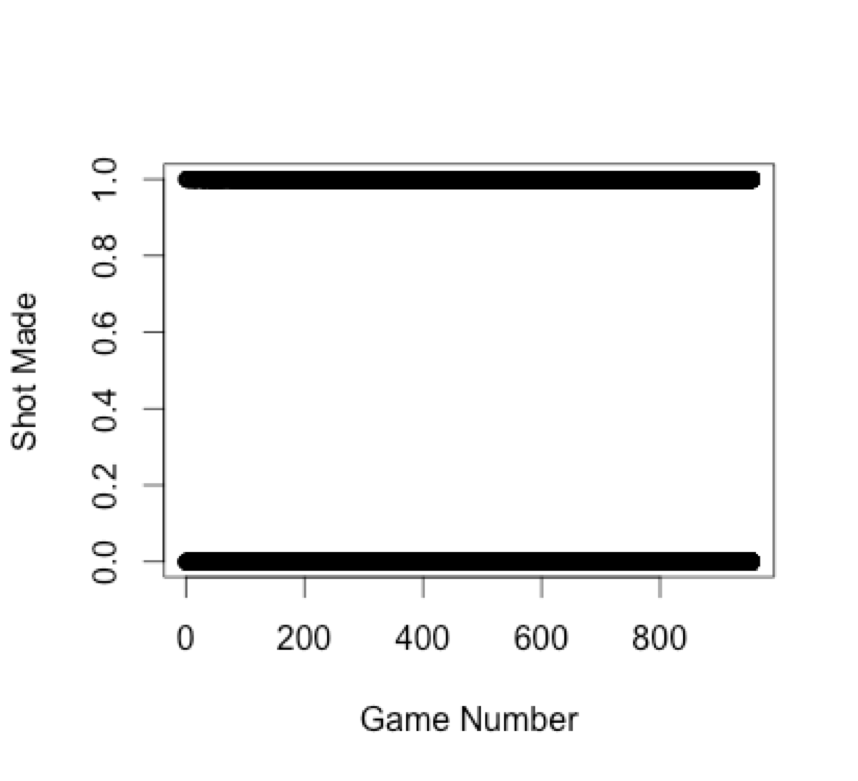
\includegraphics[width=10cm]{img/autocorrelation}
\end{center}
\hspace*{1cm}Next, we created the correlation plot below to determine if the regressor variables are highly related to one another.
\begin{center}
	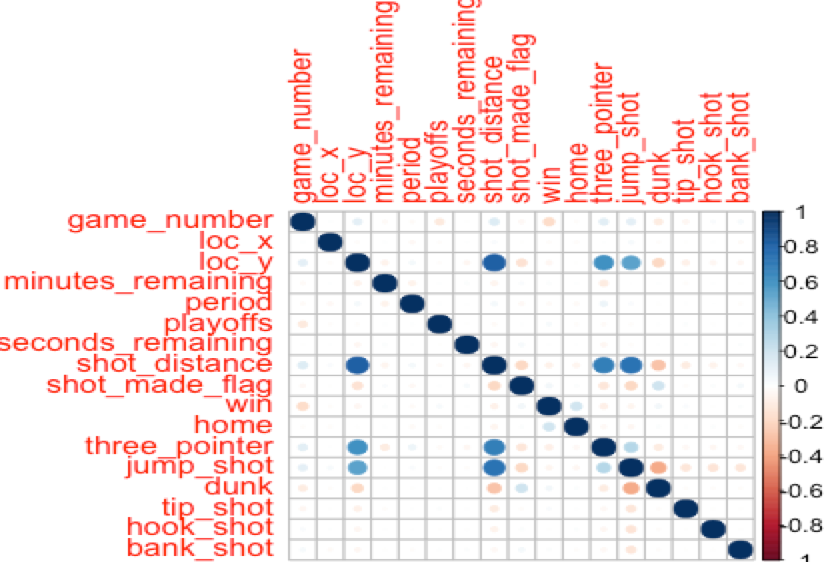
\includegraphics[width=10cm]{img/corrplot}
\end{center}
\hspace*{1cm}The above plot showed us that \texttt{shot\_distance} and \texttt{loc\_y} are the only two variables with a significantly high correlation. We measured this correlation using the \texttt{cor} command and found that it was .812. Therefore, we chose to exclude \texttt{loc\_y} from our regression model to satisfy (4), our independent regressors assumption.

\hspace*{1cm}Since we checked the fit of the model by building the logit model in R (as shown below), we ensured that our data met all logit model assumptions. 

\hspace*{1cm}To build the logit model, we used the \texttt{glm} function in R to obtain the output below (after removing the least significant variables in previous calls of \texttt{glm}): 
\begin{center}
	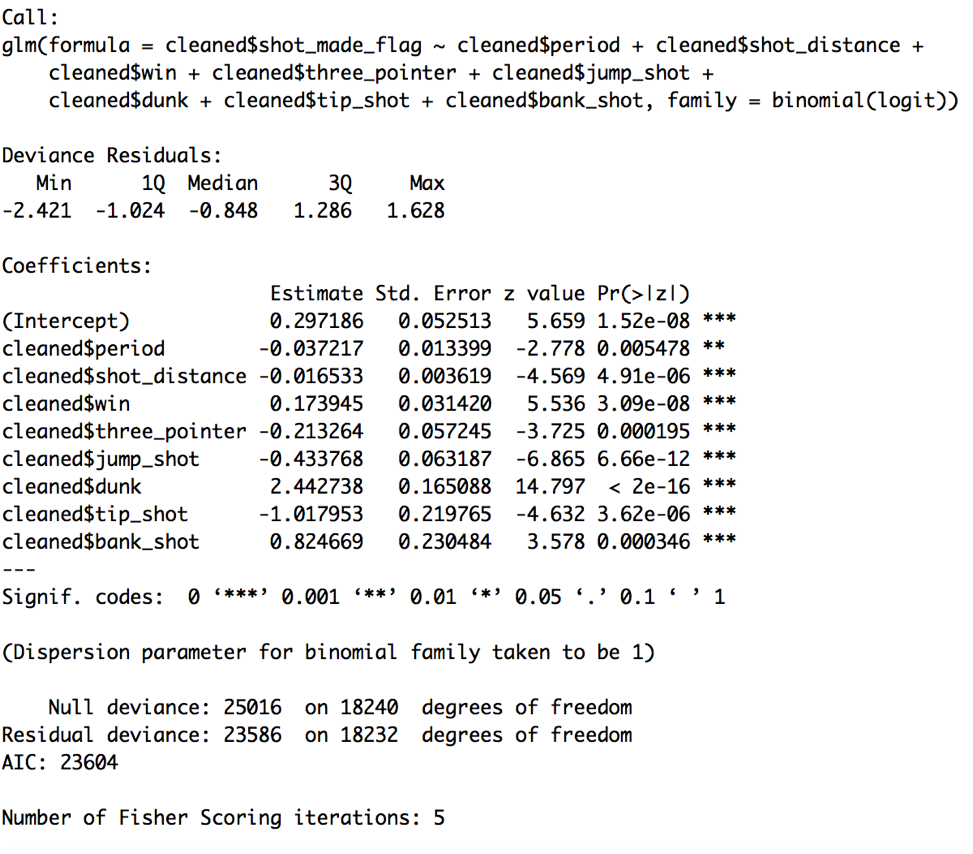
\includegraphics[width=14cm]{img/logit1}
\end{center}

\hspace*{1cm}Note that we did not include the seconds remaining variable in our model because that variable is not a measure of how many seconds were remaining absolutely in the game as one would think, but rather the number of seconds remaining in a particular minute (which could have been any minute of a quarter). This was poorly documented by Kaggle and was a source of confusion for us at first, but once we discovered the meaning of the variable, we corrected our model accordingly.

\hspace*{1cm} For the sake of comparison, we also utilized the \texttt{stepwise} command from the \texttt{Rcmdr}
package. Using the AIC criterion with a backwards stepwise regression, we obtain: 
\begin{center}
	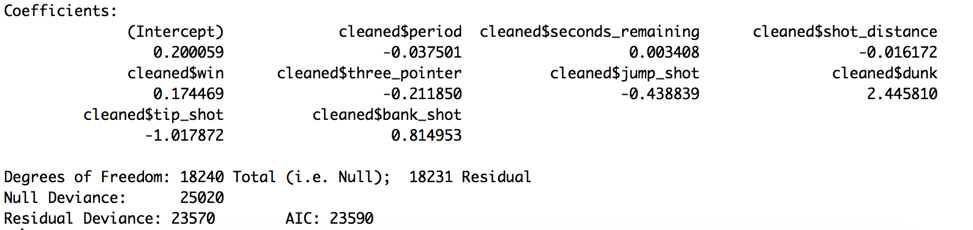
\includegraphics[width=14cm]{img/logitaic}
\end{center}
\hspace*{1cm}Using the BIC criterion to run a backwards stepwise regression with the \texttt{stepwise} command yielded:
\begin{center}
	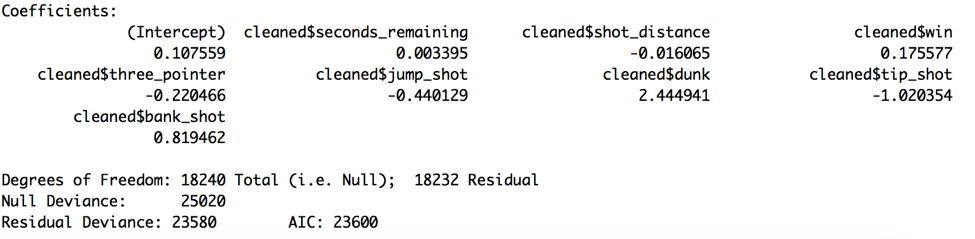
\includegraphics[width=14cm]{img/logitbic}
\end{center}
\hspace*{1cm} Despite the aforementioned issues with performing linear regression on a binary response variable, we thought it would be instructive to do so anyway for the sake of comparison with the results from the logistic model. After removing the least significant variables in a stepwise fashion, running the \texttt{lm} command produced the following result: 
\begin{center}
	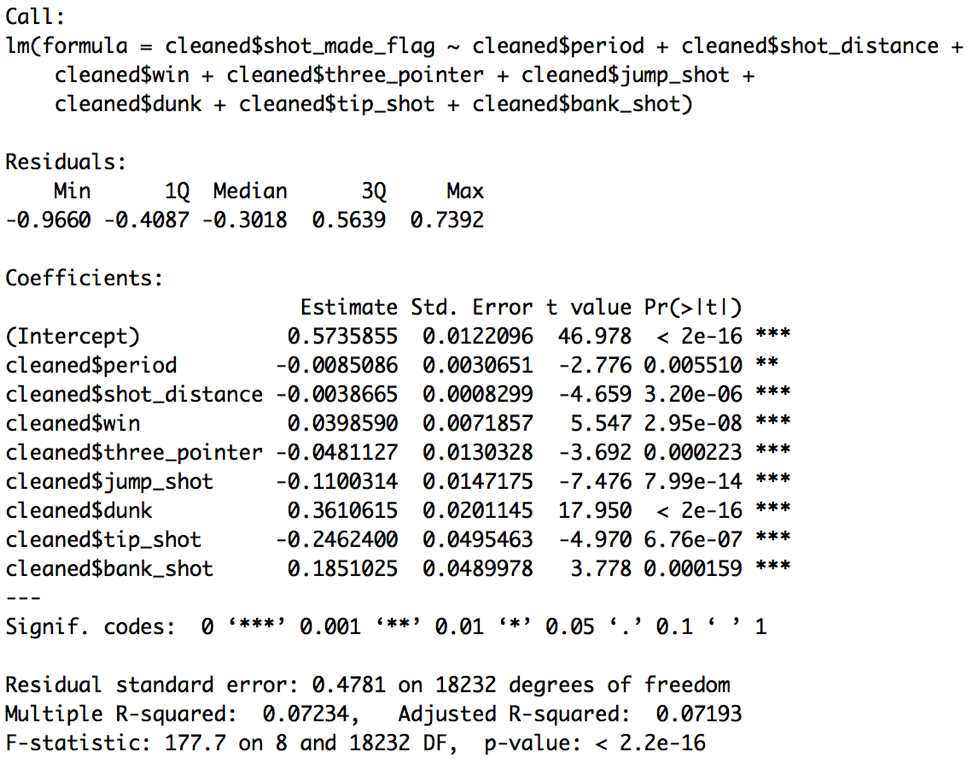
\includegraphics[width=14cm]{img/lm1}
\end{center}
\hspace*{1cm} Using the \texttt{stepwise} command in conjuction with the full linear model yielded the following result under the AIC criterion:
\begin{center}
	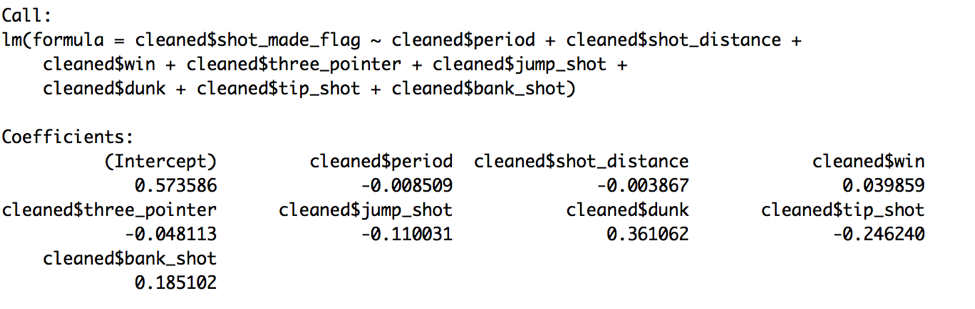
\includegraphics[width=14cm]{img/lmaic}
\end{center}
\hspace*{1cm} Under the BIC criterion, \texttt{stepwise} yielded:
\begin{center}
	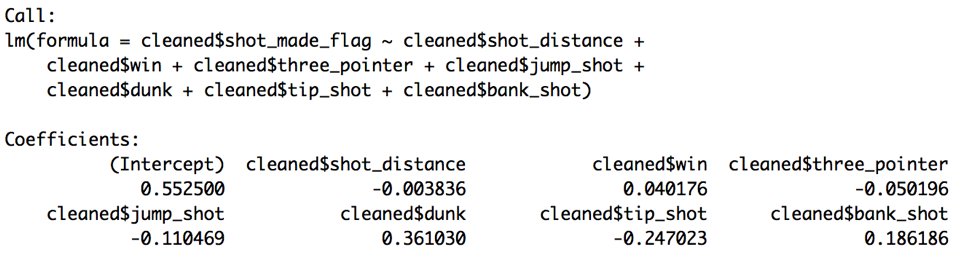
\includegraphics[width=14cm]{img/lmbic}
\end{center}
\hspace*{1cm}Interpreting the logit model was not nearly as straightforward as interpreting a linear model because, for the logit model, a one-unit increase in an independent variable was associated with a change in the log odds of the dependent variable instead of the dependent variable itself (as it would have been in a linear model). Because of this, we decided to focus primarily on interpreting the sign of the coefficients produced by the logit model.

\hspace*{1cm}For the logit models, all of the coefficients were almost exactly the same across all 3 models and they all had the same sign. The only notable difference was that the first and second models (manual backwards stepwise and AIC stepwise) included \texttt{period} while the third one did not. 

\hspace*{1cm}Based on the signs of the coefficients in the three logit models, we were able to make the following observations: 
\begin{itemize}
\item An increase in shot distance was associated with a lower probability of a successful shot. This makes sense because being farther from the basket would intuitively make a succesful shot more difficult. 
\item Having won the game a given shot was made during was associated with a higher probability that Kobe made a given shot.
\item Having a shot be a three-pointer, jump shot, or tip shot was associated with a lower probability that Kobe would make the shot. 
\item Having a shot be a dunk or a bank shot was associated with a higher probability of a successful shot. Based on the magnitudes and holding all else constant, it appears that Kobe's most accurate shot was the dunk and his least accurate shot was the tip shot. 
\item The game number, the x location of the shot, the minutes remaining, whether or not the game was a playoff game, whether or not a game was a home game, and whether or not the shot was a hook shot did not have a significant impact on the probability that Kobe made a given shot. 
\end{itemize}

\hspace*{1cm}The linear model would have failed almost every single one of our regression diagnostics so we decided that running them would be redundant. For example, the dependent variable was binary so all of our residuals would have exhibited heteroskedasticity. However, by comparing the linear model results to the logit model results, we found that the signs of the coefficients of the significant regressors agreed with the signs of the logit model coefficients, lending support to the validity of the observations derived from the logit model coefficients. 

\subsubsection{Logistic Regression on Win/Loss Data}
\hspace*{1cm}To evaluate whether or not Kobe's game performance affected the ultimate result of a given game (on average), we ran a logit regression using the \texttt{win} variable mentioned above (obtained by scraping win/loss data) against the summary statistics of Kobe's game performance. To avoid multicollinearity between our regressors, we chose to only regress \texttt{win} against \texttt{clutch\_perc} and \texttt{non\_clutch\_perc} (because these two statistics were calculated using the \texttt{shots\_made}, \texttt{shots\_taken}, \texttt{clutch\_shots\_made} and \texttt{clutch\_shots\_taken} variables, including any of these variables in the model would have caused our regressors to be extremely interdependent and therefore would have resulted in multicollinearity). Even though we had fewer observations for win/loss data than for shooting data because unique observations occurred on a game-by-game basis as opposed to on a shot-by-shot basis, our win/loss data still satisfied the assumptions necessary to run a logit regresion. 

\hspace*{1cm}Given the similar results obtained by running the \texttt{stepwise} command and manually performing a backwards stepwise regression for the shooting data, we thought it was reasonable to only perform the latter, which produced:
\begin{center}
	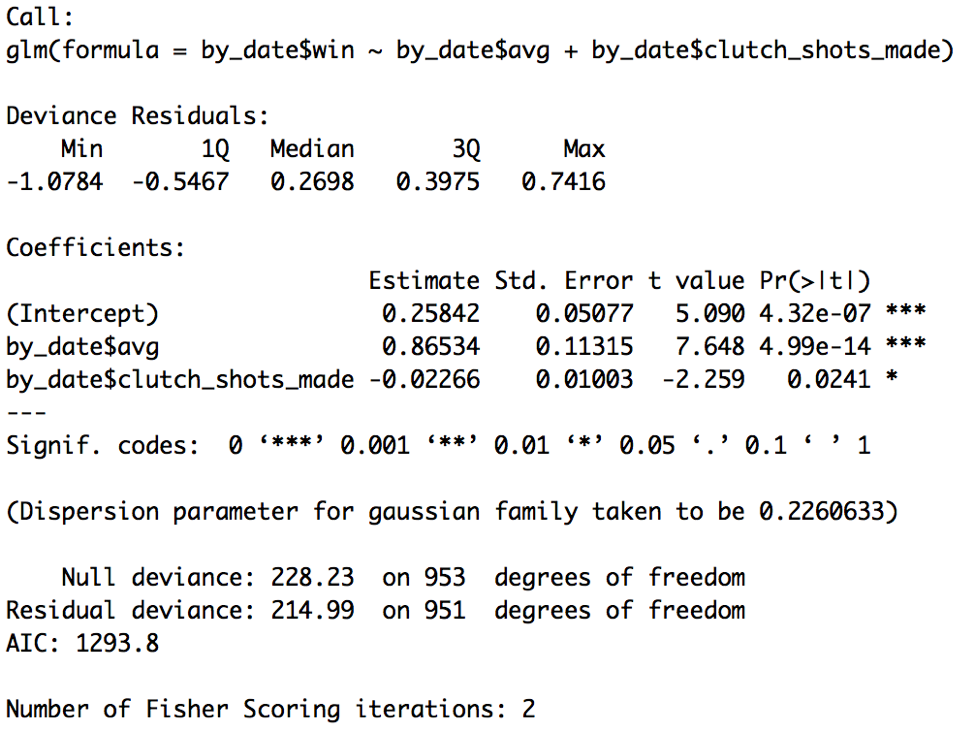
\includegraphics[scale=0.6]{img/logitwins}
\end{center}
\hspace*{1cm}According to the results above, both Kobe's average shooting percentage and clutch shooting percentage for a given game were associated with a higher probability of a Lakers win, supporting our hypothesis that Kobe's game performance significantly affected on the probability of a win. 
\subsubsection{Stationarity}
\hspace*{1cm}If a given data set is stationary, then the mean, variance, and autocorrelation do not change over time. That is, a stationary series is a flat looking series, without a trend, which has constant variance over time. Stationarity was an important consideration for us to look at because we wanted to see if Kobe's shot percentage changed somehow over time. Did injuries affect how good he was? Did aging cause his shot accuracy to fall or did experience cause it to go up? We used the \texttt{adf.test} function in R to test for stationarity. The null hypothesis was that the data was not stationary and the alternative was that the data was stationary. 
\begin{center}
	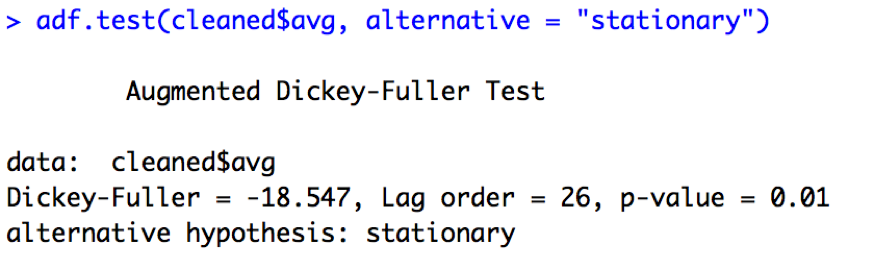
\includegraphics[scale=0.65]{img/stationarity}
\end{center}
\hspace*{1cm}Because the p-value from this test was .01, we rejected the null hypothesis in favor of the alternative hypothesis that our data was stationary at the 95\% level of confidence. Therefore, Kobe's shot accuracy seems to have remained fairly stable over time, regardless of injury. 
\subsection{Cross Validation}
\hspace*{1cm}We considered the possibility of cross validation for the logit models for shooting data and win/loss data we produced and we thought it might be interesting to see how the linear model performed against the logit model. However, because our objectives consisted mainly of predicting binary response variables, we assumed that the models predicted successes (either in terms of a succesful shot or a win) when the response variable outputs were probabilities of 0.5 or higher and that the models predicted failures if the response variable outputs were probabilities of below 0.5. Under these assumptions, the only difference between how the two types of models predicted the response variables were based solely on where the models crossed probability = 0.5. This meant that validation would have been pointless because we were not checking how close to each point we were like we were with a regular linear regression on a non-binary response variable (with residual values). Additionally, we could measure how far from 0 or 1 each response produced by the logit models was, but the logit model clearly would have had a lower overall distance because of the function was a curve as opposed to the straight line generated by the linear models. Therefore we decided that cross validation would have been inappropriate in this situation.

\section{Limitations}
\subsection{Lack of Free-Throw Data}
\hspace*{1cm}One disadvantage of the dataset we utilized was that it only considered field goals during running game time i.e. 2-point and 3-point field goals. While free throws are often considered indicative of a player's effectiveness in clutch situations, in many ways regular field goals are more impressive because, unlike with free throws, players are challenged by their opponents when taking jump shots and layups. Thus, despite this specific absence in the dataset we feel that our analysis still reveals much about Kobe's overall effectiveness in normal and higher stress clutch conditions.

\subsection{Definition of Clutch}
\hspace*{1cm}Given the amount of data we had to work with, we had to set a quantitative threshold for our definition of clutch based on the variables available to us (in this case seconds remaining and period). Different definitions of clutch could potentially yield different results. For example, another plausible interpretation of clutch could be shots made to tie or win a game in the last two minutes, which would be an interesting subject for future analysis.

\section{Challenges Faced \& Lessons Learned}
\hspace*{1cm}One challenge we faced while performing data preprocessing was that the \texttt{date} variable obtained from scraping the win-loss data originally used a long-form format (e.g, ``May 2, 2016''). When we used Excel to change the date formatting and proceeded with the data cleaning in \texttt{cleaning.R}, we noticed that some of the dates were years in the future (which is clearly beyond the realm of possibility for basketball shots already taken by Kobe Bryant). To resolve this error, we passed in the raw data obtained by the scraping process into R, and discovered that R had a parsing option for long-form dates. Using the R-formatted dates, we were able to accurately merge the win-loss data with our shooting data. 

\hspace*{1cm}On the topic of data preprocessing, we learned that real-world data can be messy to work with. The data we had to work with from Kaggle was relatively clean to begin with, but even then we had to do some nontrivial preprocessing in order to suit our analysis.

\hspace*{1cm}In terms of performing analysis, one of our main takeaways was that given a large amount of data and features, it is a challenge to determine what sort of analysis to perform. There are many more potential statistical relationships we could have explored given the richness of the data set. That said, we believe that we have performed a reasonable amount of analysis for the goal of addressing our research questions.
\section{Conclusion}
\hspace*{1cm}When considering the hypotheses we posited before performing the data analysis, our results showed a surprising mixture of evidence, supporting some of our initial beliefs while pushing back on others. For example, although increases in shot distance did lead to a decrease in field goal percentage, in terms of individual shot type tip ins were Kobe's least effective shot despite their proximity to the basket. In the context of the sport this conclusion does make sense, however, considering that of the shot types we considered players have the least control over tip ins, which are shots attempted immediately after securing an offensive rebound. 

\hspace*{1cm}Perhaps the most surprising result was Kobe's effectiveness in the clutch, as our analysis showed that contrary to our initial hypothesis Kobe was actually more effective in non-clutch as opposed to clutch situations. One potential explanation of his poorer clutch performance lies in how teams approach late-game situations. In the clutch, many teams structure their offensive strategies differently, relying on stars like Kobe to carry even more of the offensive burden in a slower pace. Conversely, opposing teams will focus their defensive strategies on shutting down those key players, which could explain why Kobe's field goal percentage was lower during those clutch periods compared with normal situations. 

\hspace*{1cm}Ultimately, however, when we consider how Kobe's performance - clutch or otherwise - related to the Lakers' chances of winning, we found our initial hypothesis was correct, with a significant positive relationship between win probability and his field goal percentage in both situations. Lastly, Kobe's reputation as a physically and mentally tough competitor held up, with injuries, home versus away games, and playoff versus regular season games not having significant effects on his overall performance. And despite some of the inherent limitations of our data, we believe that our analyses have supported Kobe's reputation as a vital cog in the Lakers' success during his long and storied career at the Staples Center. 
\begin{thebibliography}{9}
	\bibitem{bootstraptheory}
	Bret Larget.
	\textit{Chapter 3: R Bootstrap Examples}, \\\texttt{http://www.stat.wisc.edu/$\sim$larget/stat302/chap3.pdf}
	
	\bibitem{kagglecompetition}
	Kaggle. 
	\textit{Kobe Bryant Shot Selection}, \texttt{https://www.kaggle.com/c/kobe-bryant-shot-selection}

	\bibitem{forumpost}
	Kaggle. 
	\textit{Splitting of data into training and test},\\ \texttt{https://www.kaggle.com/c/DontGetKicked/forums/t/975/splitting-of-data-into-training-and-test}

	\bibitem{landofbasketball}
	Land of Basketball.com.
	\textit{Los Angeles Lakers}, \\\texttt{http://www.landofbasketball.com/teams/records\_los\_angeles\_lakers.htm}
	


\end{thebibliography}
\section*{Acknowledgements}
\hspace*{1cm}Special thanks to Phillip Huang for his kind assistance in helping us scrape win-loss data using the ``Web Scraper'' Chrome extension.

\end{document}